\begin{frame}
	\frametitle{Zusammenfassung und Ausblick}
	\begin{figure}
		\centering
		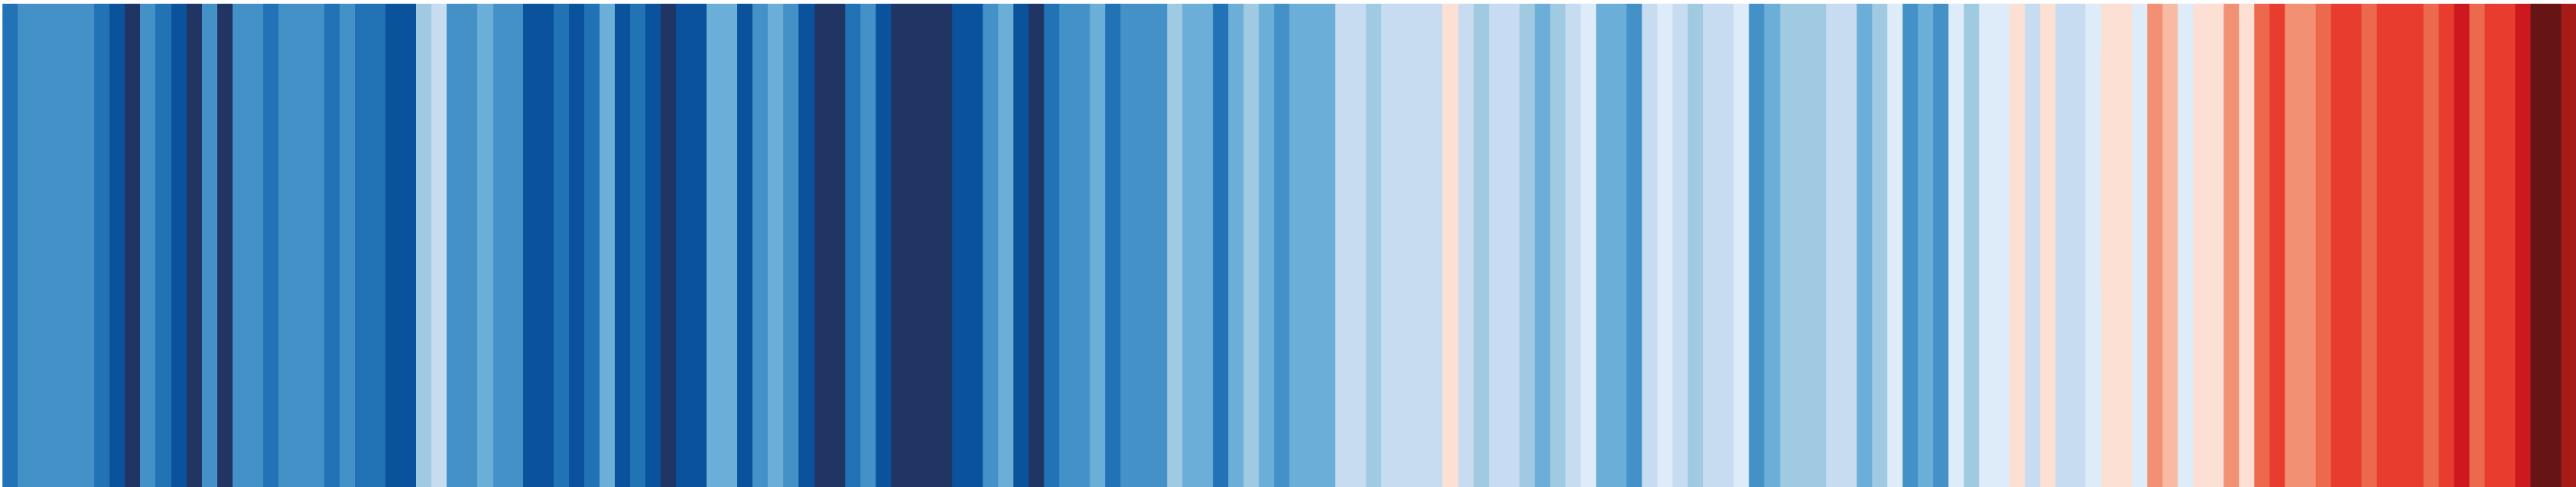
\includegraphics[width=\linewidth]{bilder/s4f-warming-stripes}
		\caption{Die Warming Stripes}
	\end{figure}
	$\rightarrow$ Die langfristige Erwärmung und Häufung extremer Wetterereignisse bedeutet eine Veränderung des Klimas!\\
	$\rightarrow$ Viele dieser Änderungen sind in Modellen der Klimaforscher relativ genau vorherzusagen. \\
	$\rightarrow$ Das Ausmaß einiger Änderungen ist aufgrund der langfristigen Effekte nicht konkret vorherzusagen, aber die Tendenz ist klar. \\
	$\rightarrow$ Der Klimawandel ist keine Naturkatastrophe, sondern menschengemacht. Wir können ihn in beide Richtungen beeinflussen. Je eher wir damit anfangen, desto leichter ist es.
\end{frame}
